% Practice Test 25 — Oklahoma Edition
% Questions: 30 (21 MC + 9 SA)
% Generated by scripts/generate_practice_tests.py

\begin{practiceQuestion}{1-3-q26}{gmc}
\begin{questionText}
The graph below shows a proportional relationship. What is the constant of proportionality?

\begin{center}
\begin{tikzpicture}[scale=0.8]
  \draw[step=1,gray!20,thin] (0,0) grid (6,6);
  \draw[thick,->] (0,0) -- (6.5,0) node[right]{\small $x$};
  \draw[thick,->] (0,0) -- (0,6.5) node[above]{\small $y$};
  \foreach \x in {1,...,6} \draw (\x,0.07) -- (\x,-0.07) node[below]{\tiny \x};
  \foreach \y in {1,...,6} \draw (0.07,\y) -- (-0.07,\y) node[left]{\tiny \y};
  \draw[thick,funBlue] (0,0) -- (6,4);
  \fill[funBlue] (0,0) circle (2.5pt);
  \fill[funBlue] (3,2) circle (2.5pt) node[above left]{\small $(3, 2)$};
  \fill[funBlue] (6,4) circle (2.5pt) node[above left]{\small $(6, 4)$};
\end{tikzpicture}
\end{center}
\end{questionText}
\choiceA{$k = \frac{1}{2}$}
\choiceB{$k = \frac{2}{3}$}
\choiceC{$k = \frac{3}{2}$}
\choiceD{$k = 2$}
\correctAnswer{B}
\explanation{Use any labeled point: $k = \frac{2}{3}$ from $(3, 2)$. Check: $\frac{4}{6} = \frac{2}{3}$ \checkmark.}
\end{practiceQuestion}

\begin{practiceQuestion}{1-6-q26}{gmc}
\begin{questionText}
The table shows the distance a bus travels over several hours. Using proportional reasoning, how far will the bus travel in $9$ hours?

\begin{center}
\begin{tabular}{|c|c|}
\hline
\textbf{Hours} & \textbf{Miles} \\ \hline
$2$ & $90$ \\ \hline
$5$ & $225$ \\ \hline
$7$ & $315$ \\ \hline
$9$ & $?$ \\ \hline
\end{tabular}
\end{center}
\end{questionText}
\choiceA{$360$ miles}
\choiceB{$385$ miles}
\choiceC{$405$ miles}
\choiceD{$450$ miles}
\correctAnswer{C}
\explanation{Rate: $90 \div 2 = 45$ mph. In $9$ hours: $45 \times 9 = 405$ miles.}
\end{practiceQuestion}

\begin{practiceQuestion}{1-7-q02}{mc}
\begin{questionText}
A building is $60$ m tall. A model uses the scale $1 : 200$. How tall is the model?
\end{questionText}
\choiceA{$30$ cm}
\choiceB{$3$ cm}
\choiceC{$300$ cm}
\choiceD{$0.3$ cm}
\correctAnswer{A}
\explanation{Divide actual by scale factor: $60 \div 200 = 0.3$ m $= 30$ cm.}
\end{practiceQuestion}

\begin{practiceQuestion}{2-1-q15}{mc}
\begin{questionText}
A library has $480$ books. If $35\%$ are fiction, how many fiction books does the library have?
\end{questionText}
\choiceA{$148$}
\choiceB{$160$}
\choiceC{$168$}
\choiceD{$172$}
\correctAnswer{C}
\explanation{$35\% = 0.35$. Multiply: $0.35 \times 480 = 168$ fiction books.}
\end{practiceQuestion}

\begin{practiceQuestion}{2-4-q18}{mc}
\begin{questionText}
Two stores sell the same $\$80$ headphones. Store A offers $25\%$ off. Store B offers $\$20$ off. Which is a better deal?
\end{questionText}
\choiceA{Store A (you pay $\$55$)}
\choiceB{Store B (you pay $\$55$)}
\choiceC{Store A (you pay $\$60$)}
\choiceD{Both stores give the same price}
\correctAnswer{D}
\explanation{Store A: $80 \times 0.75 = \$60$. Store B: $80 - 20 = \$60$. Both give the same price of $\$60$.}
\end{practiceQuestion}

\begin{practiceQuestion}{2-7-q30}{gsa}
\begin{questionText}
The bar graph shows the estimated and actual amounts of water (in liters) collected during an experiment over three days. On which day was the percent error the largest, and what was it?

\begin{center}
\begin{tikzpicture}[scale=0.5]
  \draw[thick,->] (0,0) -- (0,6.5) node[above]{\small Liters};
  \draw[thick,->] (0,0) -- (10.5,0);
  % Day 1: est 10, actual 8
  \fill[funBlue!60] (0.5,0) rectangle (1.5,5);
  \fill[funGreen!60] (1.5,0) rectangle (2.5,4);
  % Day 2: est 6, actual 5
  \fill[funBlue!60] (3.5,0) rectangle (4.5,3);
  \fill[funGreen!60] (4.5,0) rectangle (5.5,2.5);
  % Day 3: est 8, actual 10
  \fill[funBlue!60] (6.5,0) rectangle (7.5,4);
  \fill[funGreen!60] (7.5,0) rectangle (8.5,5);
  \node[below,font=\small] at (1.5,0) {Day 1};
  \node[below,font=\small] at (4.5,0) {Day 2};
  \node[below,font=\small] at (7.5,0) {Day 3};
  \foreach \y/\lab in {1/2,2/4,3/6,4/8,5/10,6/12} {
    \draw (-0.1,\y) -- (0.1,\y) node[left,font=\small,xshift=-2pt] {\lab};
  }
  \node[above,font=\scriptsize,funBlue] at (1,5) {$10$};
  \node[above,font=\scriptsize,funGreen!80!black] at (2,4) {$8$};
  \node[above,font=\scriptsize,funBlue] at (4,3) {$6$};
  \node[above,font=\scriptsize,funGreen!80!black] at (5,2.5) {$5$};
  \node[above,font=\scriptsize,funBlue] at (7,4) {$8$};
  \node[above,font=\scriptsize,funGreen!80!black] at (8,5) {$10$};
  % Legend
  \fill[funBlue!60] (0.5,6.3) rectangle (1,6.7);
  \node[right,font=\scriptsize] at (1.1,6.5) {Estimated};
  \fill[funGreen!60] (3.5,6.3) rectangle (4,6.7);
  \node[right,font=\scriptsize] at (4.1,6.5) {Actual};
\end{tikzpicture}
\end{center}
\end{questionText}
\correctAnswer{Day 1 with $25\%$ error}
\explanation{Day 1: $|10-8|/8 = 25\%$. Day 2: $|6-5|/5 = 20\%$. Day 3: $|8-10|/10 = 20\%$. Day 1 has the largest percent error at $25\%$.}
\end{practiceQuestion}

\begin{practiceQuestion}{2-8-q20}{sa}
\begin{questionText}
Bank A has a $\$4$ monthly fee. Bank B has no monthly fee. How much do you save per year at Bank B?
\end{questionText}
\correctAnswer{$\$48$}
\explanation{$4 \times 12 = \$48$ saved per year.}
\end{practiceQuestion}

\begin{practiceQuestion}{3-1-q22}{sa}
\begin{questionText}
A submarine is at $-200$ meters. It rises $200$ meters. What is its new depth?
\end{questionText}
\correctAnswer{$0$ meters (sea level)}
\explanation{$-200 + 200 = 0$. Rising $200$ meters from $-200$ meters brings the submarine to sea level.}
\end{practiceQuestion}

\begin{practiceQuestion}{4-1-q04}{mc}
\begin{questionText}
Evaluate $2a + 7$ when $a = -3$.
\end{questionText}
\choiceA{$13$}
\choiceB{$1$}
\choiceC{$-13$}
\choiceD{$-1$}
\correctAnswer{B}
\explanation{Substitute: $2(-3) + 7 = -6 + 7 = 1$.}
\end{practiceQuestion}

\begin{practiceQuestion}{4-2-q04}{mc}
\begin{questionText}
Simplify $3y + 8 - 5y - 2$.
\end{questionText}
\choiceA{$8y + 6$}
\choiceB{$-2y + 6$}
\choiceC{$2y - 6$}
\choiceD{$-2y + 10$}
\correctAnswer{B}
\explanation{Combine variable terms: $3y - 5y = -2y$. Combine constants: $8 - 2 = 6$. Result: $-2y + 6$.}
\end{practiceQuestion}

\begin{practiceQuestion}{5-3-q29}{gsa}
\begin{questionText}
The total area of the figure below is $84$ square cm. Find $x$.

\begin{center}
\begin{tikzpicture}[scale=0.5]
  % 6 identical rectangles side by side
  \foreach \i in {0,...,5} {
    \draw[thick,fill=funBlue!15] (\i*2,0) rectangle (\i*2+2,3);
  }
  \draw[<->] (0,-0.7) -- (12,-0.7);
  \node[below] at (6,-0.7) {$6$ rectangles, each width $(x + 1)$ cm};
  \draw[<->] (-0.7,0) -- (-0.7,3);
  \node[left] at (-0.7,1.5) {$2$ cm};
  \node at (6,4.2) {Total area $= 84$ sq. cm};
\end{tikzpicture}
\end{center}
\end{questionText}
\correctAnswer{$x = 6$}
\explanation{Total area $= 6 \times 2 \times (x + 1) = 84$. So $12(x + 1) = 84$. Divide by $12$: $x + 1 = 7$. Subtract $1$: $x = 6$.}
\end{practiceQuestion}

\begin{practiceQuestion}{5-4-q14}{mc}
\begin{questionText}
Solve $0.6x - 2.4 = 1.2$.
\end{questionText}
\choiceA{$x = 6$}
\choiceB{$x = -2$}
\choiceC{$x = 2$}
\choiceD{$x = 0.6$}
\correctAnswer{A}
\explanation{Add $2.4$: $0.6x = 3.6$. Divide by $0.6$: $x = 6$. Check: $0.6(6) - 2.4 = 3.6 - 2.4 = 1.2$ \checkmark.}
\end{practiceQuestion}

\begin{practiceQuestion}{5-5-q29}{gsa}
\begin{questionText}
The balance scale tips to the left. Write and solve the inequality that describes this situation.

\begin{center}
\begin{tikzpicture}[scale=0.7]
  % Tilted beam (left side heavier)
  \draw[thick] (0,-0.5) -- (-0.4,-1.2) -- (0.4,-1.2) -- cycle;
  \draw[thick] (-4.5,0.5) -- (4.5,-0.5);
  % Left pan (lower = heavier)
  \draw[thick] (-4.5,0.5) -- (-5.3,0) -- (-3.7,0) -- (-4.5,0.5);
  \draw[thick,fill=funBlue!20] (-5.3,0) -- (-5.3,-0.4) -- (-3.7,-0.4) -- (-3.7,0) -- cycle;
  \node at (-4.5,-0.2) {$2x + 8$};
  % Right pan (higher = lighter)
  \draw[thick] (4.5,-0.5) -- (5.3,-1) -- (3.7,-1) -- (4.5,-0.5);
  \draw[thick,fill=funOrange!20] (3.7,-1) -- (3.7,-1.4) -- (5.3,-1.4) -- (5.3,-1) -- cycle;
  \node at (4.5,-1.2) {$20$};
\end{tikzpicture}
\end{center}
\end{questionText}
\correctAnswer{$2x + 8 > 20$; $x > 6$}
\explanation{The left side is heavier (tips down), so $2x + 8 > 20$. Subtract $8$: $2x > 12$. Divide by $2$: $x > 6$.}
\end{practiceQuestion}

\begin{practiceQuestion}{5-6-q18}{mc}
\begin{questionText}
Solve $6 - 2x \leq -4$ and describe the graph.
\end{questionText}
\choiceA{Closed circle at $5$, shade right}
\choiceB{Open circle at $5$, shade right}
\choiceC{Closed circle at $5$, shade left}
\choiceD{Closed circle at $-5$, shade right}
\correctAnswer{A}
\explanation{Subtract $6$: $-2x \leq -10$. Divide by $-2$ and flip: $x \geq 5$. Closed circle at $5$, shade right.}
\end{practiceQuestion}

\begin{practiceQuestion}{6-2-q18}{mc}
\begin{questionText}
A drawing uses $1$ cm $= 5$ km. A road is $7$ cm long. Another map shows the same road as $3.5$ cm. What is the scale of the second map?
\end{questionText}
\choiceA{$1$ cm $= 2.5$ km}
\choiceB{$1$ cm $= 5$ km}
\choiceC{$1$ cm $= 10$ km}
\choiceD{$1$ cm $= 17.5$ km}
\correctAnswer{C}
\explanation{Actual road: $7 \times 5 = 35$ km. New scale: $35 \div 3.5 = 10$. So the second map uses $1$ cm $= 10$ km.}
\end{practiceQuestion}

\begin{practiceQuestion}{6-3-q19}{sa}
\begin{questionText}
Can a triangle have sides $10$ cm, $6$ cm, and $3$ cm? Explain why or why not.
\end{questionText}
\correctAnswer{No}
\explanation{$6 + 3 = 9 < 10$. The two shorter sides cannot span the longest side. The triangle inequality is not satisfied.}
\end{practiceQuestion}

\begin{practiceQuestion}{6-4-q13}{mc}
\begin{questionText}
Can a triangle have angles $90°$, $100°$, and $-10°$?
\end{questionText}
\choiceA{Yes, it is a right triangle}
\choiceB{Yes, because the sum is $180°$}
\choiceC{No, because an angle cannot be negative}
\choiceD{No, because the sum is not $180°$}
\correctAnswer{C}
\explanation{Although $90 + 100 + (-10) = 180$, every angle in a triangle must be greater than $0°$. A negative angle is impossible.}
\end{practiceQuestion}

\begin{practiceQuestion}{6-5-q29}{gsa}
\begin{questionText}
The diagram shows a cylinder with radius $4$ cm and height $9$ cm. A vertical cut is made through the center. Describe the cross-section and give its dimensions.

\begin{center}
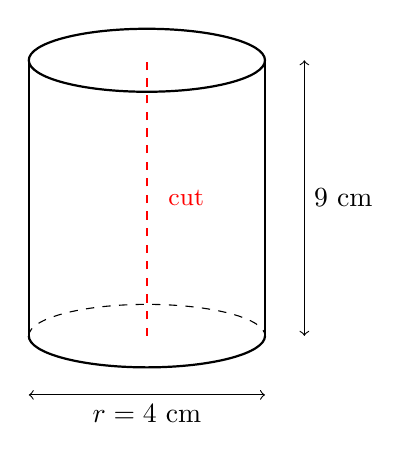
\begin{tikzpicture}[scale=0.5]
  % Cylinder
  \draw[thick] (-3,0) -- (-3,7);
  \draw[thick] (3,0) -- (3,7);
  \draw[thick] (-3,0) arc[start angle=180,end angle=360,x radius=3,y radius=0.8];
  \draw[dashed] (-3,0) arc[start angle=180,end angle=0,x radius=3,y radius=0.8];
  \draw[thick] (-3,7) arc[start angle=180,end angle=360,x radius=3,y radius=0.8];
  \draw[thick] (-3,7) arc[start angle=180,end angle=0,x radius=3,y radius=0.8];
  % Vertical cut line
  \draw[thick,red,dashed] (0,0) -- (0,7);
  \node[right,red] at (0.3,3.5) {\small cut};
  % Labels
  \draw[<->] (-3,-1.5) -- (3,-1.5);
  \node[below] at (0,-1.5) {$r = 4$ cm};
  \draw[<->] (4,0) -- (4,7);
  \node[right] at (4,3.5) {$9$ cm};
\end{tikzpicture}
\end{center}
\end{questionText}
\correctAnswer{Rectangle; $8$ cm by $9$ cm}
\explanation{A vertical cut through the center of a cylinder produces a rectangle. Width = diameter = $2 \times 4 = 8$ cm. Height = $9$ cm.}
\end{practiceQuestion}

\begin{practiceQuestion}{6-6-q10}{mc}
\begin{questionText}
Two angles are supplementary. One is $25°$ more than the other. What are the two angles?
\end{questionText}
\choiceA{$65°$ and $115°$}
\choiceB{$77.5°$ and $102.5°$}
\choiceC{$80°$ and $100°$}
\choiceD{$75°$ and $105°$}
\correctAnswer{B}
\explanation{Let the smaller be $x$. Then $x + (x + 25) = 180$. Combine: $2x + 25 = 180$. Solve: $2x = 155$, $x = 77.5°$. The other: $77.5 + 25 = 102.5°$.}
\end{practiceQuestion}

\begin{practiceQuestion}{7-4-q05}{mc}
\begin{questionText}
A rectangular yard is $20$ m by $15$ m. A circular flower bed with radius $3$ m is in the center. What is the area of the yard NOT covered by the flower bed? Use $\pi \approx 3.14$.
\end{questionText}
\choiceA{$271.74$ m$^2$}
\choiceB{$300$ m$^2$}
\choiceC{$328.26$ m$^2$}
\choiceD{$28.26$ m$^2$}
\correctAnswer{A}
\explanation{Yard: $20 \times 15 = 300$ m$^2$. Circle: $3.14 \times 9 = 28.26$ m$^2$. Remaining: $300 - 28.26 = 271.74$ m$^2$.}
\end{practiceQuestion}

\begin{practiceQuestion}{7-5-q01}{mc}
\begin{questionText}
What is the surface area of a cube with side length $4$ cm?
\end{questionText}
\choiceA{$16$ cm$^2$}
\choiceB{$64$ cm$^2$}
\choiceC{$96$ cm$^2$}
\choiceD{$24$ cm$^2$}
\correctAnswer{C}
\explanation{A cube has $6$ faces. $SA = 6s^2 = 6 \times 16 = 96$ cm$^2$.}
\end{practiceQuestion}

\begin{practiceQuestion}{7-6-q11}{mc}
\begin{questionText}
A triangular prism has a triangular base with legs $5$ cm and $12$ cm (right triangle). The prism is $15$ cm long. What is the volume?
\end{questionText}
\choiceA{$150$ cm$^3$}
\choiceB{$300$ cm$^3$}
\choiceC{$450$ cm$^3$}
\choiceD{$900$ cm$^3$}
\correctAnswer{C}
\explanation{$B = \frac{1}{2} \times 5 \times 12 = 30$ cm$^2$. $V = 30 \times 15 = 450$ cm$^3$.}
\end{practiceQuestion}

\begin{practiceQuestion}{8-1-q23}{sa}
\begin{questionText}
A radio station asks listeners to call in and vote for their favorite song. Explain why this is not a random sample.
\end{questionText}
\correctAnswer{Only listeners who choose to call participate, so it is voluntary and biased}
\explanation{Voluntary response samples are biased because people with strong opinions are more likely to respond.}
\end{practiceQuestion}

\begin{practiceQuestion}{8-3-q28}{gmc}
\begin{questionText}
The histograms show the distribution of weekly study hours for two groups.

\begin{center}
\begin{tikzpicture}[scale=0.55]
  % Group A
  \node[font=\small\bfseries] at (3.5,5) {Group A};
  \draw[thick,->] (0,0) -- (0,4.5);
  \draw[thick,->] (0,0) -- (7.5,0);
  \node[below,font=\small] at (3.5,-0.5) {Hours};
  \foreach \y in {1,2,3,4} { \draw (-0.1,\y) -- (0.1,\y); \node[left,font=\tiny] at (0,\y) {$\y$}; }
  \fill[funBlue!60] (0.5,0) rectangle (1.5,1);
  \fill[funBlue!60] (1.5,0) rectangle (2.5,2);
  \fill[funBlue!60] (2.5,0) rectangle (3.5,4);
  \fill[funBlue!60] (3.5,0) rectangle (4.5,3);
  \fill[funBlue!60] (4.5,0) rectangle (5.5,2);
  \fill[funBlue!60] (5.5,0) rectangle (6.5,1);
  \node[below,font=\tiny] at (1,0) {$2$};
  \node[below,font=\tiny] at (2,0) {$4$};
  \node[below,font=\tiny] at (3,0) {$6$};
  \node[below,font=\tiny] at (4,0) {$8$};
  \node[below,font=\tiny] at (5,0) {$10$};
  \node[below,font=\tiny] at (6,0) {$12$};
\end{tikzpicture}
\hspace{1cm}
\begin{tikzpicture}[scale=0.55]
  % Group B
  \node[font=\small\bfseries] at (3.5,5) {Group B};
  \draw[thick,->] (0,0) -- (0,4.5);
  \draw[thick,->] (0,0) -- (7.5,0);
  \node[below,font=\small] at (3.5,-0.5) {Hours};
  \foreach \y in {1,2,3,4} { \draw (-0.1,\y) -- (0.1,\y); \node[left,font=\tiny] at (0,\y) {$\y$}; }
  \fill[funGreen!60] (0.5,0) rectangle (1.5,3);
  \fill[funGreen!60] (1.5,0) rectangle (2.5,4);
  \fill[funGreen!60] (2.5,0) rectangle (3.5,2);
  \fill[funGreen!60] (3.5,0) rectangle (4.5,2);
  \fill[funGreen!60] (4.5,0) rectangle (5.5,1);
  \fill[funGreen!60] (5.5,0) rectangle (6.5,1);
  \node[below,font=\tiny] at (1,0) {$2$};
  \node[below,font=\tiny] at (2,0) {$4$};
  \node[below,font=\tiny] at (3,0) {$6$};
  \node[below,font=\tiny] at (4,0) {$8$};
  \node[below,font=\tiny] at (5,0) {$10$};
  \node[below,font=\tiny] at (6,0) {$12$};
\end{tikzpicture}
\end{center}

Which group tends to study more hours per week?
\end{questionText}
\choiceA{Group A, because most of its data is at higher values}
\choiceB{Group B, because most of its data is at higher values}
\choiceC{Group A, because it has more spread}
\choiceD{They study the same amount}
\correctAnswer{A}
\explanation{Group A's histogram peaks at $6$--$8$ hours, while Group B's peaks at $2$--$4$ hours. Group A tends to study more.}
\end{practiceQuestion}

\begin{practiceQuestion}{8-4-q16}{mc}
\begin{questionText}
Group A: $\{60, 65, 70, 75, 80\}$. Group B: $\{40, 55, 70, 85, 100\}$. Both have a mean of $70$. Which group is more variable?
\end{questionText}
\choiceA{Group A}
\choiceB{Group B}
\choiceC{They are equally variable}
\choiceD{Cannot be determined}
\correctAnswer{B}
\explanation{Group A range $= 20$, Group B range $= 60$. Group B's data is far more spread out.}
\end{practiceQuestion}

\begin{practiceQuestion}{8-5-q23}{sa}
\begin{questionText}
The data set is: $28, 31, 33, 36, 40, 42$. What is the median?
\end{questionText}
\correctAnswer{$34.5$}
\explanation{$6$ values: median $= \frac{33+36}{2} = \frac{69}{2} = 34.5$.}
\end{practiceQuestion}

\begin{practiceQuestion}{8-7-q02}{mc}
\begin{questionText}
Which data display is best for showing how data changes over time?
\end{questionText}
\choiceA{Circle graph}
\choiceB{Line graph}
\choiceC{Stem-and-leaf plot}
\choiceD{Box plot}
\correctAnswer{B}
\explanation{A line graph connects data points over time, making trends easy to see.}
\end{practiceQuestion}

\begin{practiceQuestion}{9-4-q26}{gmc}
\begin{questionText}
Look at the spinner below. Which probability model correctly represents this spinner?

\begin{center}
\begin{tikzpicture}[scale=1.2]
  \fill[funRed!50] (0,0) -- (0:1.5) arc (0:180:1.5) -- cycle;
  \fill[funBlue!50] (0,0) -- (180:1.5) arc (180:270:1.5) -- cycle;
  \fill[funGreen!50] (0,0) -- (270:1.5) arc (270:360:1.5) -- cycle;
  \draw[thick] (0,0) circle (1.5);
  \draw[thick] (0,0) -- (0:1.5);
  \draw[thick] (0,0) -- (180:1.5);
  \draw[thick] (0,0) -- (270:1.5);
  \node at (90:0.8) {\textbf{Red}};
  \node at (225:0.8) {\textbf{Blue}};
  \node at (315:0.8) {\textbf{Green}};
\end{tikzpicture}
\end{center}
\end{questionText}
\choiceA{$P(\text{Red}) = \frac{1}{3}$, $P(\text{Blue}) = \frac{1}{3}$, $P(\text{Green}) = \frac{1}{3}$}
\choiceB{$P(\text{Red}) = \frac{1}{2}$, $P(\text{Blue}) = \frac{1}{4}$, $P(\text{Green}) = \frac{1}{4}$}
\choiceC{$P(\text{Red}) = \frac{1}{4}$, $P(\text{Blue}) = \frac{1}{4}$, $P(\text{Green}) = \frac{1}{2}$}
\choiceD{$P(\text{Red}) = \frac{1}{2}$, $P(\text{Blue}) = \frac{1}{2}$, $P(\text{Green}) = 0$}
\correctAnswer{B}
\explanation{Red covers half the spinner ($180\degree$), while Blue and Green each cover a quarter ($90\degree$ each). This is a non-uniform model.}
\end{practiceQuestion}

\begin{practiceQuestion}{9-6-q15}{mc}
\begin{questionText}
Two dice are rolled. What is the probability that the product (not the sum) of the two numbers is $12$?
\end{questionText}
\choiceA{$\frac{2}{36}$}
\choiceB{$\frac{4}{36}$}
\choiceC{$\frac{3}{36}$}
\choiceD{$\frac{6}{36}$}
\correctAnswer{B}
\explanation{Pairs with product $12$: $(2,6), (6,2), (3,4), (4,3)$ — that is $4$ out of $36$. $P = \frac{4}{36} = \frac{1}{9}$.}
\end{practiceQuestion}

\begin{practiceQuestion}{9-7-q10}{mc}
\begin{questionText}
A student simulates rolling two dice $36$ times to see how often the sum is $7$. They get a sum of $7$ a total of $8$ times. How does this compare to the expected number?
\end{questionText}
\choiceA{Expected: $6$; the simulation result ($8$) is slightly higher}
\choiceB{Expected: $6$; the simulation result ($8$) is much higher}
\choiceC{Expected: $12$; the simulation result ($8$) is lower}
\choiceD{Expected: $7$; the simulation result ($8$) is exact}
\correctAnswer{A}
\explanation{$P(\text{sum} = 7) = \frac{6}{36} = \frac{1}{6}$. Expected: $36 \times \frac{1}{6} = 6$. The simulation gave $8$, slightly above expected.}
\end{practiceQuestion}
